% Para definir o tipo de documento, descomente apenas
% uma das linhas "\documentclass" abaixo

% comentar uma linha significa colocar "%"
% descomentar uma linha significa remover o "%"

%\documentclass[msc]{on}     % dissertação de mestrado
\documentclass[dsc]{on}     % tese de doutorado
%\documentclass[dscexam]{on} % exame de qualificação
%\documentclass[reportd]{on} % relatório feito durante o doutorado
%\documentclass[reportm]{on} % relatório feito durante o mestrado

% pacotes utilizados
\usepackage[utf8]{inputenc}
\usepackage{amsmath,amssymb}
\usepackage{hyperref}
\usepackage{enumerate} %para gerar listas numeradas
\usepackage{graphicx}  %para figuras eps
\usepackage{subfigure} %para figuras múltimas, com (a), (b), (c), etc.

% os dois comandos estão com problema e deverão ser
% corrigidos futuramente
%\makelosymbols
%\makeloabbreviations

\begin{document}

  % Título em português
  \title{Título}
  
  % Título em inglês
  \foreigntitle{Title}
  
  % Autor
  \author{Nome do(a) Autor(a)}{Sobrenome}

  % Orientador(a)
  \advisor{Dra.}{Nome da orientadora}{Sobrenome}
  %\advisor{Dr.}{Nome do orientador}{Sobrenome}

  % Co-orientadores (pode ser mais de um)
  \coadvisor{Dra.}{Nome da Co-orientadora}{Sobrenome}
  \coadvisor{Dr.}{Nome do Co-orientador}{Sobrenome}

  % Examinadores (caso seja um relatório, não modifique as linhas "\examiner")
  \examiner{Dra.}{Nome da Examinadora}{Sobrenome}
  \examiner{Dr.}{Nome do Examinador}{Sobrenome}
  \examiner{Dra.}{Nome da Examinadora}{Sobrenome}
  \examiner{Dr.}{Nome do Examinador}{Sobrenome}
  \examiner{Dra.}{Nome da Examinadora}{Sobrenome}

  % Programa de Pós-Graduação 
  \program{GEO}
  %\program{ASTRO}
  
  % Data (mês e ano)
  \date{03}{2017}

  % Palavras-chave
  \keyword{Primeira palavra-chave}
  \keyword{Segunda palavra-chave}
  \keyword{Terceira palavra-chave}

  \maketitle

  % caso seja um relatório, comente as quatro (4) próximas linhas
  \frontmatter     % folha de rosto
  \makecatalog     % ficha catalogŕafica
  \dedication{Dedicat\'oria (opcional).}

  % dedicatória
  \chapter*{Agradecimentos}

Agradecimentos (opcional).
 % agradecimentos
  
  \begin{abstract}

Este projeto propõe ...

\end{abstract}


  \begin{foreignabstract}

In this work, we propose ... 

\end{foreignabstract}


  \tableofcontents   % sumário
  \listoffigures     % lista de figuras (opcional)
  \listoftables      % lista de tabelas (opcional)

  % os dois comandos estão com problema e deverão ser
  % corrigidos futuramente
  %\printlosymbols
  %\printloabbreviations

  \mainmatter

  % As linhas "\include" abaixo incluem os capítulos no documento.
  % Edite os arquivos "chapxx.tex" de acordo com as suas necessidades.
  % No presente documento, são incluídos seis capítulos, mas é possível
  % utilizar quantos capítulos forem necessários.
  \chapter{Introdução}

\textbf{OBS0: Testado com o MikTex 2.9 em Windows e TeX Live 2015/Debian no Ubuntu, ambos rodando o PDFLaTex para geração diretamente do PDF da tese (anexado como exemplo). Como editor, indicamos o WinEdt.}

OBS1: Segundo a norma de formatação de teses e disserta{\c c}\~oes do
Programa de Pós-graduação em Geofísica do Observatório Nacional (PPG-ON)
é obrigatório que toda abreviatura seja definida na primeira vez que é
utilizada, mas não é obrigatório colocar uma lista de abreviações no preâmbulo.
Entretanto, é altamente indicado que se coloque uma lista de abreviação no
preâmbulo, com todas as abreviações utilizadas no trabalho, uma vez que isto
torna o texto mais claro.

EXEMPLO.

Um exemplo de utilização de abreviação é dado na seguir: O Método das Diferenças Finitas
(MDF\abbrev{MDF}{Método dos Diferenças Finitas}) é um dos métodos numéricos mais eficientes
para a resolução de equações diferenciais...

Repare que, na primeira vez que a abreviação ocorre no texto, basta utilizar o comando
``\verb|\abbrev|'' para descrever a abreviação, sendo tal abreviação colocada automaticamente
e uma listagem de abreviações no preâmbulo do texto.

Do mesmo modo, pode-se definir os símbolos com o comando ``\verb|\symbl|'', tal como o
conjunto dos números reais $\mathbb{R}$ e o conjunto vazio $\emptyset$.
\symbl{$\mathbb{R}$}{Conjunto dos n\'umeros reais}
\symbl{$\emptyset$}{Conjunto vazio}

Após isto, antes de compilar o código com pdflatex por exemplo, é necessário rodar o make index
para gerar as listas, por exemplo, através dos seguinte comandos na linha de comando:

\verb|makeindex -s on.ist -o thesis.lab thesis.abx|

\verb|makeindex -s on.ist -o thesis.los thesis.syx|


  \chapter{Contexto Geológico}

Para ilustrar a completa ades\~ao ao estilo de cita{\c c}\~oes e listagem de
refer\^encias bibliogr\'aficas, a Tabela~\ref{tab:citation} apresenta cita{\c
c}\~oes de alguns dos trabalhos, utilizando o estilo alfabético (default). Para
utilização do estilo numérico, deve-se utilizar a opção number da classe ON, ou seja,
basta usar \verb|\documentclass[dsc, numbers]{on}|.

\begin{table}[h]
\caption[Exemplos de tabela (texto do índice)]{Exemplos de tabela mostrando os comandos para
  cita{\c c}\~oes utilizando o comando padr\~ao \texttt{\textbackslash citep} do \LaTeX\ e
  o comando \texttt{\textbackslash citet},
  fornecido pelo pacote \texttt{natbib}.}
\label{tab:citation}
\centering
{\footnotesize
\begin{tabular}{|c|c|c|}
  \hline
  Tipo da Publica{\c c}\~ao & \verb|\citep| & \verb|\citet|\\
  \hline
  Livro & \citep{book-example} & \citet{book-example}\\
  Artigo & \citep{article-example} & \citet{article-example}\\
  Relat\'orio & \citep{techreport-example} & \citet{techreport-example}\\
  Relat\'orio & \citep{techreport-exampleIn} & \citet{techreport-exampleIn}\\
  Anais de Congresso & \citep{inproceedings-example} &
    \citet{inproceedings-example}\\
  S\'eries & \citep{incollection-example} & \citet{incollection-example}\\
  Em Livro & \citep{inbook-example} & \citet{inbook-example}\\
  Disserta{\c c}\~ao de mestrado & \citep{mastersthesis-example} &
    \citet{mastersthesis-example}\\
  Tese de doutorado & \citep{phdthesis-example} & \citet{phdthesis-example}\\
  \hline
\end{tabular}}
\end{table}

\section{seção 1}


  \chapter{Objetivos geral e espec\'{i}ficos}

  \chapter{Metodologia}

Um exemplo de utilização de equações matemáticas é apresentado abaixo na Equação~\ref{eq:nome1}:
\begin{equation}
\label{eq:nome1}E=mc^2
\end{equation}

Para um conjunto de equações, como as Equações~\ref{eq:nome2}-\ref{eq:nome3}:
\begin{eqnarray}
\label{eq:nome2} & & \;\;\;\;\; \rho \partial_t v_i
 - \partial_j \tau_{ij} = f_i\\
\label{eq:nome3} & &
\partial_t \tau_{ij}-c_{ijkl}\partial_l v_{k}=-\partial_tg_{ij},
\end{eqnarray}


Um exemplo de utilização de figuras no \LaTeX é apresentado a seguir: na
Figura~\ref{fig:caption1} é mostrado uma figura-exemplo contendo um snapshot
de uma propagação de ondas elásticas em um meio anisotrópico.
\begin{figure}[hbt]
\centering 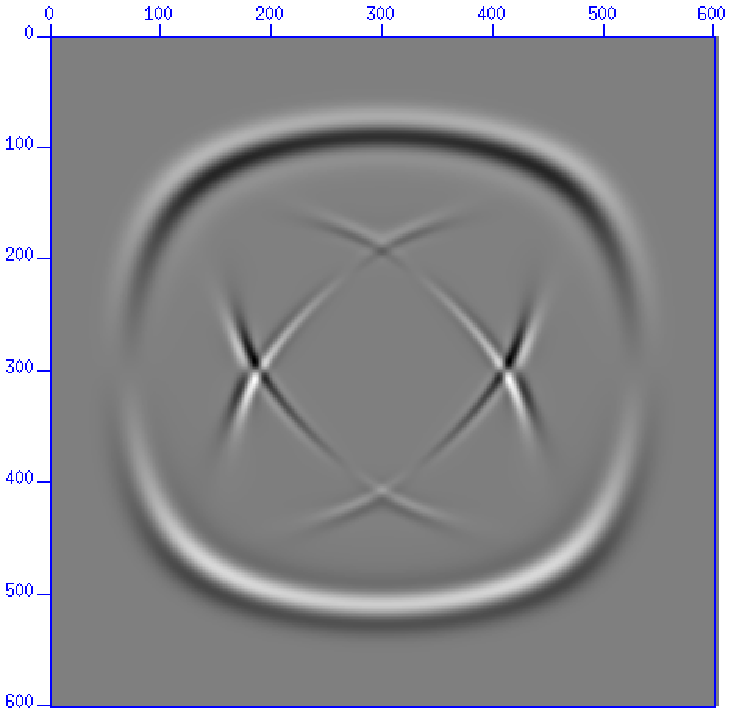
\includegraphics[width=6.5cm,height=6.5cm]{Figs/snap}
\caption[Exemplo de figura simples (texto do índice).]{Exemplo de figura simples:
modelagem elástica de um meio anisotrópico.}
\label{fig:caption1}
\end{figure}

Exemplo de utilização de figuras múltiplas é apresentado na Figura~\ref{fig:cc}
abaixo. Podemos referenciar cada uma das figuras, por exemplo a Figura~\ref{fig:cc_nr} ou
a Figura~\ref{fig:cc_cerjan}.
\begin{figure}[hbt]
\centering \subfigure[Condição de contorno não reflexiva
(CCNR).]{\label{fig:cc_nr}
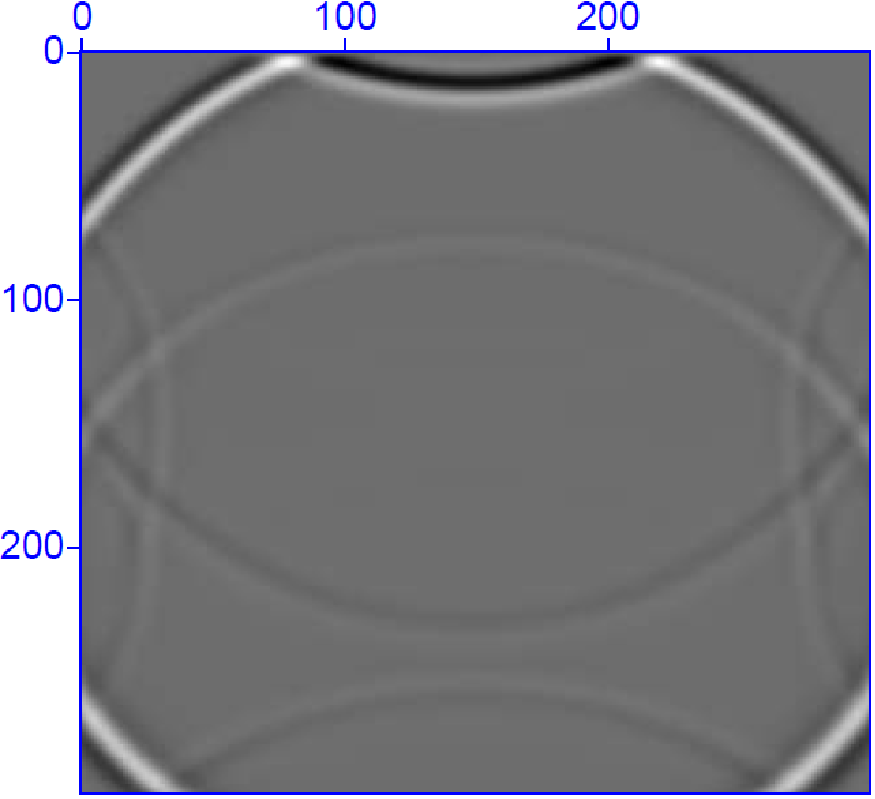
\includegraphics[width=6.5cm,height=6.5cm]
{Figs/cc_nr}} \qquad \subfigure[Camadas de amortecimento +
CCNR.]{\label{fig:cc_cerjan}
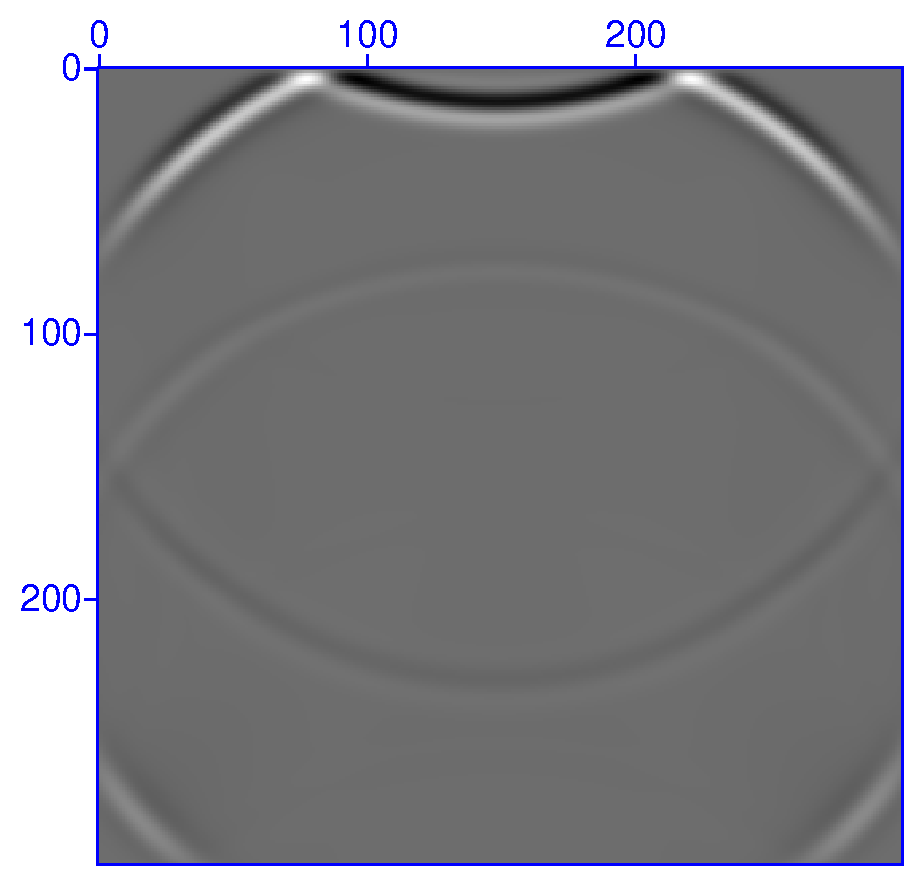
\includegraphics[width=6.5cm,height=6.5cm]{Figs/cerjan}}
\caption[Exemplo de múltiplas figuras (texto do índice).]{Exemplo de múltiplas
figuras: modelagem
acústica mostrando efeito da aplicação da CCNR e camadas de amortecimento
aplicadas nas bordas (menos na superfície). Aplica-se em (a) as CCNR de
Reynolds e em (b) as camadas de amortecimento mais CCNR de Reynolds.}
\label{fig:cc}
\end{figure}

Repare para que o exemplo acima funcione corretamente, é necessário a utilização do pacote``\verb|\usepackage{subfigure}|'', declarado no preambulo do documento principal. Para tal, este pacete deve estar instalado no LaTex utilizado para processar o documento. Indicamos a utilização do MikTex (gratuito) mais atual com editor WinEdt (pago).
  \chapter{Resultados e Discussões}

  \chapter{Cronograma detalhado}

Em geral, o cronograma de execu\c{c}\~{a}o das atividades a serem feitas ao longo de um projeto
de pesquisa \'{e} apresentado na forma de tabela. \'{E} importante ressaltar que o projeto de pesquisa 
de mestrado \'{e} \'{e} avaliado no terceiro trimestre do primeiro ano. Nesta \'{e}poca, espera-se que
algumas atividades previstas no projeto j\'{a} tenham sido executadas.

A tabela abaixo usa alguns s\'{i}mbolos do pacote \verb|pifont| (\url{https://en.wikibooks.org/wiki/LaTeX/Special_Characters#Other_symbols}). O comando \verb|\ding{número}| insere um determinado s\'{i}mbolo.

\begin{table}[h]
\caption[]{Exemplo ilustrativo de um Cronograma de atividades a serem desenvolvidas durante o mestrado.
As siglas T1$-$T8 indicam os trimestres. A c\'{e}lulas em cinza representam o planejamento inicial. Os símbolos \ding{52} e \ding{45} indicam, respectivamente atividades conclu\'{i}das e em andamento. \\}
\label{tab:cronograma}
\centering
{\footnotesize
\begin{tabular}{|c|c|c|c|c|c|c|c|c|}
  \hline
  Atividade & T1 & T2 & T3 & T4 & T5 & T6 & T7 & T8 \\
  \hline
  Revis\~{a}o bibliogr\'{a}fica & \cellcolor{gray}\ding{52} & \cellcolor{gray}\ding{52} & & & & & & \\  
  Disciplinas & \cellcolor{gray}\ding{52} & \cellcolor{gray}\ding{52} & & & & & & \\
  Processamento dos dados 1 & & \cellcolor{gray}\ding{52} & \cellcolor{gray}\ding{45} & \cellcolor{gray} & & & & \\
  Processamento dos dados 2 & & \cellcolor{gray}\ding{52} & \cellcolor{gray}\ding{45} & \cellcolor{gray} & & & & \\
  Interpreta\c{c}\~{a}o dos resultados & & & & \cellcolor{gray} & \cellcolor{gray} & \cellcolor{gray} & \cellcolor{gray} & \\
  Escrita da disserta\c{c}\~{a}o & & & & & & & \cellcolor{gray} & \cellcolor{gray} \\
  \hline
\end{tabular}}
\end{table}

De acordo com o cronograma acima, as atividades ``Revis\~{a}o bibliogr\'{a}fica" e ``Disciplinas" j\'{a} foram conclu\'{i}das e as atividades ``Processamento dos dados 1" e ``Processamento dos dados 2" foram iniciadas no trimestre T2.


  \backmatter

  % estilo de citações por ordem alfabética (defaut da classe ONTeX)
  \bibliographystyle{on-plain}
  \bibliography{references}

  \appendix
  % A linha "\include" abaixo inclui um capítulo de apêndice.
  % Edite o arquivo "appenA.tex" de acordo com as suas necessidades.
  % É possível incluir outros capítulos de apêndice. Para tanto,
  % crie outros arquivos "appenX.tex", de acordo com as suas necessidades,
  % e inclua-os no documento utilizando "\include{appenX}".
  \chapter{Algumas Demonstrações}

Aqui devem entrar demonstrações mais longas, revisões de conceitos mais básicos
ou qualquer detalhe pertinente que não seja adequado para o corpo da
dissertação/tese.


\end{document} 